\section{Google Fusion Table Javascript Library (GftLib)}
\label{gftlib-js}
Die Google Fusion Table Library (GftLib) ist eine von uns entwickelte JavaScript-Bibliothek, welche die Kommunikation mit dem Google Fusion Table SQL API (siehe Abschnitt \ref{sql-api}) vereinfacht. Sie hilft dabei SQL-Abfragen zu erstellen und per \gls{AJAX} an das API zu versenden. Zudem kümmert sich die Library um die Authentifizierung via \gls{OAuth}, so dass auch schreibende Zugriffe oder Zugriffe auf private Tabellen möglich sind.

Die Bibliothek hat Abhängigkeiten zu jQuery\footnote{\url{http://jquery.com/}} (für einige Hilfsfunktionen) sowie dem Google API JavaScript Client\footnote{\url{http://code.google.com/p/google-api-javascript-client/}} (für die Authentifizierung und das Abschicken der Requests).

Die Bibliothek besteht aus 2 Klassen (GftLib und SqlBuilder). Die GftLib ist das API zum Client und steuert dementsprechend die Requests und die Authentifizierung. Der SqlBuilder ist eine Hilfsklasse, welche es erlaubt auf einfach Art und Weise SQL Befehle zu generieren.

\subsection{Beispiel}
In folgendem Beispiel sieht man die GftLib und den SqlBuilder im Einsatz. Zuerst werden alle benötigten Werte initialisiert (Zeilen 1-4), dann wird die Ausgabefunktion \inlinecode{printer} definiert, welche später als Callback-Funktion dient für den Request. Das heisst, dass die Funktion aufgerufen wird, sobald die Antwort der Abfrage zurückkommt. 

Mit der Funktion \inlinecode{convertToObject()} wird die Antwort von Google Fusion Tables in eine für den Benutzer angenehmere Form umgewandelt. Das Resultat der Fusion Tables kommt in der Form eines zweidimensionalen Arrays zurück, jeweils für jeden Datensatz alle abgefragten Felder. Die Funktion erstellt jeweils pro Datensatz ein Objekt, welches die angefragten Felder als Properties hat. So kann man mit deren Namen auf ihre Werte zugreifen (z.B. \inlinecode{places[i].name} oder \inlinecode{places[i].population}).

In diesem Beispiel wird das SQL Query direkt in der Funktion \inlinecode{execSelect()} erzeugt, welche dazu den SqlBuilder verwendet.

\lstset{language=JavaScript}
\begin{lstlisting}
var tableId = '1LWXSMsZINyfjAKGqeS-822wi4WmlaGmmvh20Ujw';
var gft = new GftLib();
var resultList = document.getElementById("result");

var printer = function(data) {
	var places = gft.convertToObject(data);

	for (var i = 0; i < places.length; i++) {
		var listElem = document.createElement('li');
		listElem.innerHTML = 'Place: ' + places[i].name + ' / Population: ' + places[i].population;
		resultList.appendChild(listElem);
	}
}

gft.execSelect(printer, {table:tableId, fields:['name', 'population']});
\end{lstlisting}

\subsection{Abhängigkeiten}
\begin{longtable}{|p{0.3\threecelltabwidth}|p{0.2\threecelltabwidth}|p{0.5\threecelltabwidth}|}
\hline 
\textbf{Library} & \textbf{Version} & \textbf{Verwendung} \\ 
\hline 
jQuery & 1.7.1-min & Helper-Funktionen und \gls{AJAX}-Requests für den OAuthTokenService  \\ 
\hline 
Google APIs Client Library & ALPHA release & \gls{AJAX}-Requests an das Google API und Authentifizierung \\ 
\hline 
\end{longtable} 

\subsection{Methoden}
\subsubsection{GftLib}
\begin{longtable}{|p{0.3\threecelltabwidth}|p{0.2\threecelltabwidth}|p{0.5\threecelltabwidth}|}
\hline 
\textbf{Methode} & \textbf{Beschreibung} & \textbf{Parameter} \\ 
\hline 
\inlinecode{execQuery( callback, query )} &  Führt eine SQL-Abfrage aus & 
\begin{itemize}[noitemsep, nosep, leftmargin=12pt, before*={\mbox{}\vspace{-\baselineskip}}, after*={\mbox{}\vspace{-\baselineskip}}]
\item \inlinecode{callback} (Funktion): Callback-Methode welche nach Beendigung der Methode aufgerufen wird. 
\item \inlinecode{query} (String): SQL-Query
\end{itemize} \\ 
\hline 
\inlinecode{execSql( callback, sql )} & Führt einen beliebigen SQL-Befehl aus & 
\begin{itemize}[noitemsep, nosep, leftmargin=12pt, before*={\mbox{}\vspace{-\baselineskip}}, after*={\mbox{}\vspace{-\baselineskip}}]
\item \inlinecode{callback}: Callback-Methode welche nach Beendigung der Methode aufgerufen wird. 
\item \inlinecode{sql}: SQL-Befehl
\end{itemize} \\ 
\hline 
\inlinecode{execSelect( callback, options )} & Führt eine \inlinecode{SELECT}-Abfrage aus & 
\begin{itemize}[noitemsep, nosep, leftmargin=12pt, before*={\mbox{}\vspace{-\baselineskip}}, after*={\mbox{}\vspace{-\baselineskip}}]
\item \inlinecode{callback}: Callback-Methode welche nach Beendigung der Methode aufgerufen wird.
\item \inlinecode{options}: Parameter-Objekt für \inlinecode{SqlBuilder.selectStmt()}
\end{itemize} \\ 
\hline
\inlinecode{execInsert( callback, options )} & Führt einen \inlinecode{INSERT}-Befehl aus & 
\begin{itemize}[noitemsep, nosep, leftmargin=12pt, before*={\mbox{}\vspace{-\baselineskip}}, after*={\mbox{}\vspace{-\baselineskip}}]
\item \inlinecode{callback}: Callback-Methode welche nach Beendigung der Methode aufgerufen wird.
\item \inlinecode{options}: Parameter-Objekt für \inlinecode{SqlBuilder.insertStmt()}
\end{itemize} \\ 
\hline
\inlinecode{execUpdate( callback, options )} & Führt einen \inlinecode{UPDATE}-Befehl aus &
\begin{itemize}[noitemsep, nosep, leftmargin=12pt, before*={\mbox{}\vspace{-\baselineskip}}, after*={\mbox{}\vspace{-\baselineskip}}]
\item \inlinecode{callback}: Callback-Methode welche nach Beendigung der Methode aufgerufen wird. 
\item \inlinecode{options}: Parameter-Objekt für \inlinecode{SqlBuilder.updateStmt()}
\end{itemize} \\ 
\hline 
\inlinecode{execDelete( callback, options )} & Führt einen \inlinecode{DELETE}-Befehl aus & 
\begin{itemize}[noitemsep, nosep, leftmargin=12pt, before*={\mbox{}\vspace{-\baselineskip}}, after*={\mbox{}\vspace{-\baselineskip}}]
\item \inlinecode{callback}: Callback-Methode welche nach Beendigung der Methode aufgerufen wird.
\item \inlinecode{options}: Parameter-Objekt für \inlinecode{SqlBuilder.deleteStmt()} 
\end{itemize} \\ 
\hline 
\inlinecode{getTableDescription( callback, options )} & Führt eine \inlinecode{DESCRIBE}-Abfrage aus & 
\begin{itemize}[noitemsep, nosep, leftmargin=12pt, before*={\mbox{}\vspace{-\baselineskip}}, after*={\mbox{}\vspace{-\baselineskip}}]
\item \inlinecode{callback}: Callback-Methode welche nach Beendigung der Methode aufgerufen wird. 
\item \inlinecode{options}: Parameter-Objekt für \inlinecode{SqlBuilder.describeStmt()}
\end{itemize} \\
\hline 
\inlinecode{createView( callback, options )} & Führt einen \inlinecode{CREATE VIEW}-Befehl aus & 
\begin{itemize}[noitemsep, nosep, leftmargin=12pt, before*={\mbox{}\vspace{-\baselineskip}}, after*={\mbox{}\vspace{-\baselineskip}}]
\item \inlinecode{callback}: Callback-Methode welche nach Beendigung der Methode aufgerufen wird. 
\item \inlinecode{options}: Parameter-Objekt für \inlinecode{SqlBuilder.createViewStmt()} 
\end{itemize} \\ 
\hline 
\inlinecode{convertToObject( gftData )} & Konvertiert das Resultat einer Abfrage in sprechende Objekte & 
\begin{itemize}[noitemsep, nosep, leftmargin=12pt, before*={\mbox{}\vspace{-\baselineskip}}, after*={\mbox{}\vspace{-\baselineskip}}]
\item \inlinecode{gftData}: Antwort auf einen SQL Befehl von Google Fusion Tables
\end{itemize} \\ 
\hline 
\end{longtable} 

\subsubsection{SqlBuilder}
Die Methoden des SqlBuilders nehmen jeweils ein Parameter-Objekt\footnote{\url{http://www.refactoring.com/catalog/introduceParameterObject.html}} entgegen und erstellen daraus SQL-Befehle, welche dann als Input für die GftLib gebraucht werden können.

\begin{longtable}{|p{0.3\threecelltabwidth}|p{0.2\threecelltabwidth}|p{0.5\threecelltabwidth}|}
\hline 
\textbf{Methode} & \textbf{Beschreibung} & \textbf{Parameter} \\ 
\hline
\inlinecode{selectStmt( options )} & Generiert ein \inlinecode{SELECT} Statement & 
\inlinecode{options}: Parameter-Objekt mit folgenden Feldern:
\begin{itemize}[noitemsep]
\item \inlinecode{fields}: Array von Feldernamen (Default *)
\item \inlinecode{table}: ID der Tabelle oder View
\item \inlinecode{conditions}: Array von Bedingungen für die \inlinecode{WHERE}-Klausel 
\end{itemize}\\
\hline
\inlinecode{insertStmt( options )} & Generiert ein \inlinecode{INSERT} Statement & 
\inlinecode{options}: Parameter-Objekt mit folgenden Feldern:
\begin{itemize}[noitemsep]
\item \inlinecode{fields}: Array von Feldernamen (Default *)
\item \inlinecode{table}: ID der Tabelle oder View
\item \inlinecode{values}: Array von Werten (in der gleichen Reihenfolge wie \inlinecode{fields})
\end{itemize}\\
\hline
\inlinecode{updateStmt( options )} & Generiert ein \inlinecode{UPDATE} Statement & 
\inlinecode{options}: Parameter-Objekt mit folgenden Feldern:
\begin{itemize}[noitemsep]
\item \inlinecode{fields}: Array von Feldernamen (Default *)
\item \inlinecode{table}: ID der Tabelle oder View
\item \inlinecode{values}: Array von Werten (in der gleichen Reihenfolge wie \inlinecode{fields})
\item \inlinecode{conditions}: Array von Bedingungen für die \inlinecode{WHERE}-Klausel
\end{itemize}\\
\hline
\inlinecode{deleteStmt( options )} & Generiert ein \inlinecode{DELETE} Statement & 
\inlinecode{options}: Parameter-Objekt mit folgenden Feldern:
\begin{itemize}[noitemsep]
\item \inlinecode{table}: ID der Tabelle oder View
\item \inlinecode{conditions}: Array von Bedingungen für die \inlinecode{WHERE}-Klausel
\end{itemize}\\
\hline
\inlinecode{describeStmt( options )} & Generiert ein \inlinecode{DESCRIBE} Statement & 
\inlinecode{options}: Parameter-Objekt mit folgenden Feldern:
\begin{itemize}[noitemsep]
\item \inlinecode{table}: ID der Tabelle oder View
\end{itemize}\\
\hline
\inlinecode{createViewStmt( options )} & Generiert ein \inlinecode{CREATE VIEW} Statement & 
\inlinecode{options}: Parameter-Objekt mit folgenden Feldern:
\begin{itemize}[noitemsep]
\item \inlinecode{viewName}: Name der neuen View
\item \inlinecode{query}: Ein SQL-Query, das der View zugrunde liegt
\end{itemize}\\
\hline
\end{longtable}

\subsection{Implementation}
\begin{figure}[H]
	\centering
	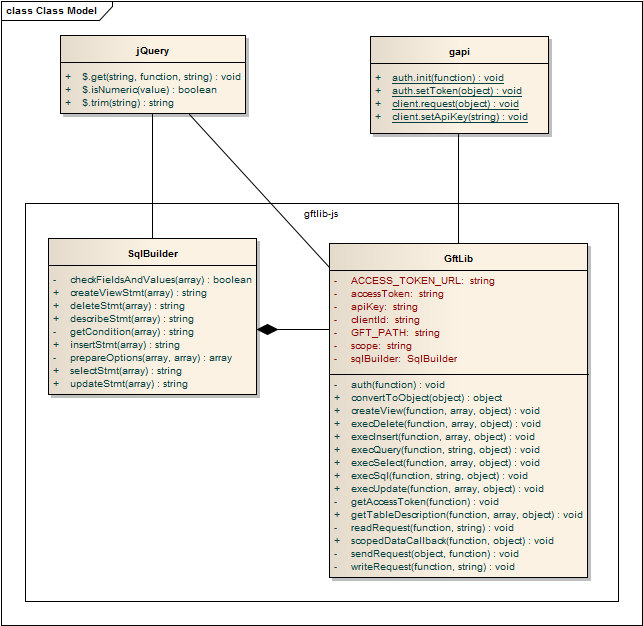
\includegraphics[width=\textwidth]{images/gftlib-js/gftlibjs-classmodel}
	\caption{GftLib Klassendiagramm}
	\label{gftlibjs-classmodel}
\end{figure}
\todo[inline]{GftLib: Implementierung?}